%!TEX root = ../thesis.tex
%*******************************************************************************
%****************************** Second Chapter *********************************
%*******************************************************************************

\chapter{Results}

As described in the previous section \todo{Link ?}, the \ttbar production cross section is measured using a template fit.
The cross section is first measured in the visible phase space requiring a dileptonic decay with the two leptons meeting the requirements of $\pt (lead) > 25 \GeV, \pt (sublead) > 20\GeV$, $\abs{\eta} < 2.4$ 
and $\mll > 20 \GeV$ .
The result for the visible cross section is:

\begin{eqnarray*}
\sigma^{vis}_{\ttbar} & = & \resultxsecvismain. 
\end{eqnarray*}

The cross section is then extrapolated to the full phase space, resulting in:

 \begin{eqnarray*}
\sigma_{\ttbar} & = & \resultxsecmain.
\end{eqnarray*}

In the following the results are described in more detail, starting with the fitted distributions in Section \ref{sec:results_templates}.

A breakdown of the systematic uncertainties is given in Section \ref{sec:results_uncert}.
It also includes a description of the pulls and constraints on the nuisance parameters as given by the results of the fit.

Finally the cross section measurement is compared to the theory prediction as well as to previous results in Section \ref{sec:results_comp}.

\section{Post-Fit Templates}
\label{sec:results_templates}

The results of the measurement of the \ttbar cross section can be applied to the distributions used in the fit, including the fitted values for the
nuisance parameters and their constraints. The nuisance parameters are applied to the templates following the interpolation described in Section \ref{sec:xsec_stat}.
All nuisance parameters are considered including those related to the normalization of the background templates.

The resulting distributions are shown in Figures \ref{fig:lh_emu_postfitdistr8}, \ref{fig:lh_mumu_postfitdistr8} and \ref{fig:lh_ee_postfitdistr8}, with the background processes
being merged into one contribution.




\begin{figure}[htbp!]
  \begin{center}
    \resizebox{0.32 \textwidth}{!}{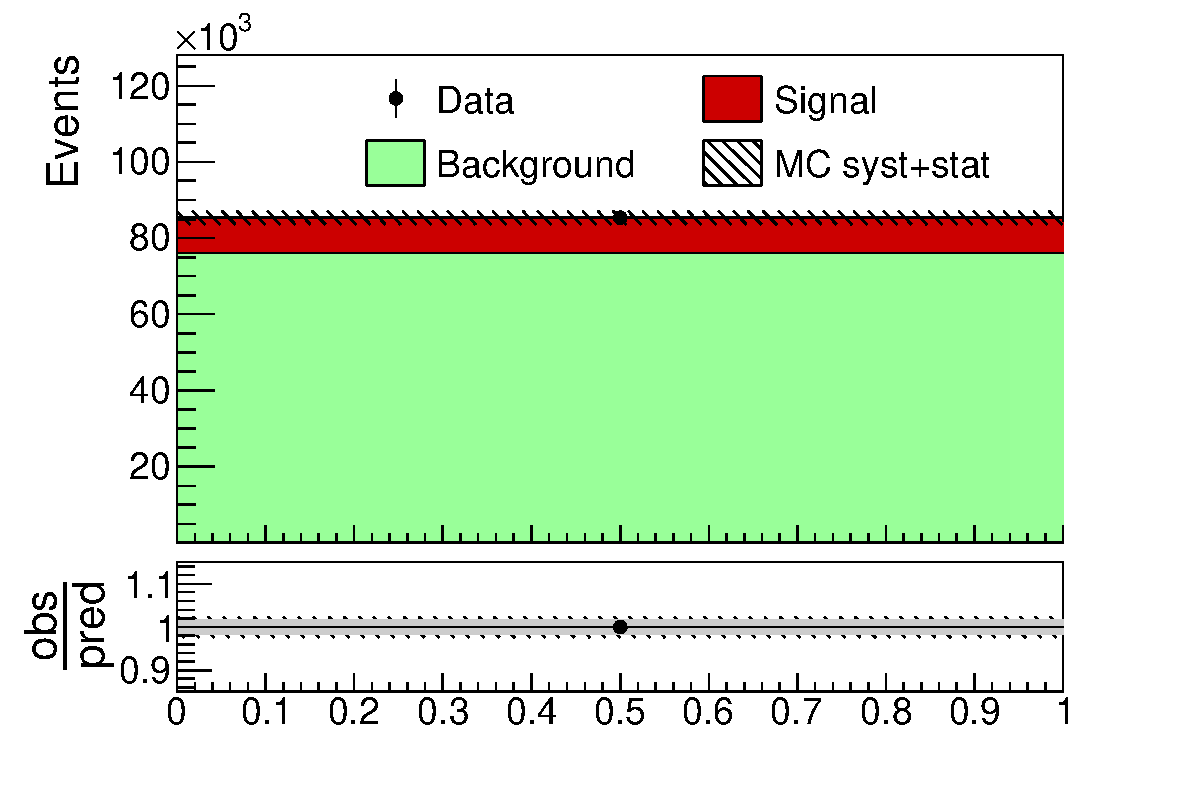
\includegraphics{Results/Figures/FitPlots/emu/total_0,0_b_jets_step_8_postfit.pdf}}
    \resizebox{0.32 \textwidth}{!}{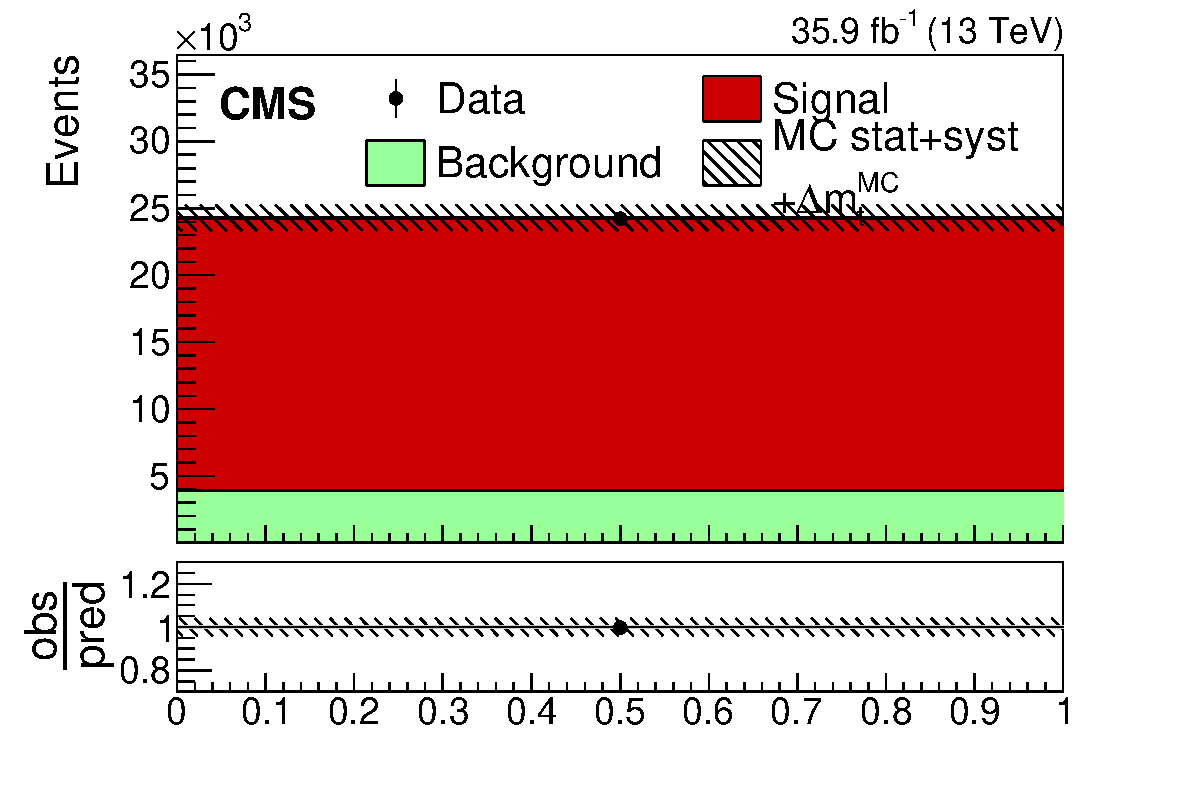
\includegraphics{Results/Figures/FitPlots/emu/total_1,0_b_jets_step_8_postfit.pdf}}
    \resizebox{0.32 \textwidth}{!}{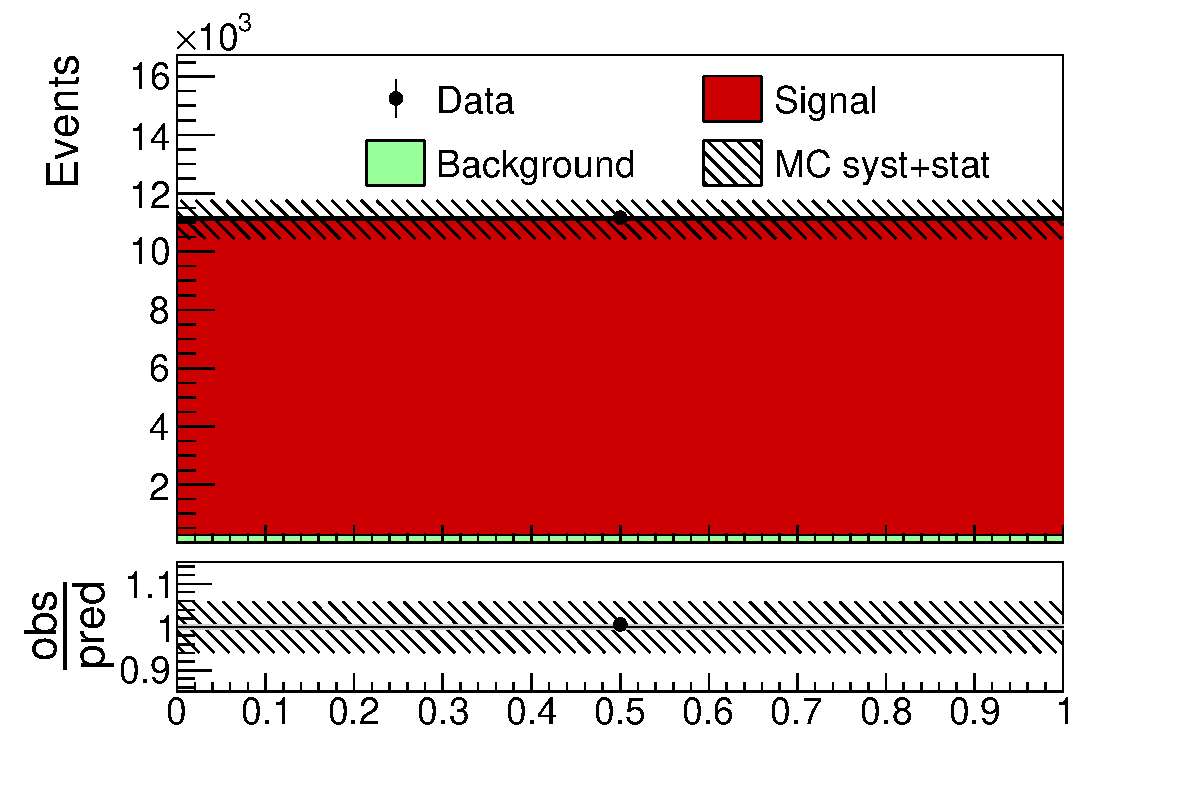
\includegraphics{Results/Figures/FitPlots/emu/total_2,0_b_jets_step_8_postfit.pdf}}

    \resizebox{0.32 \textwidth}{!}{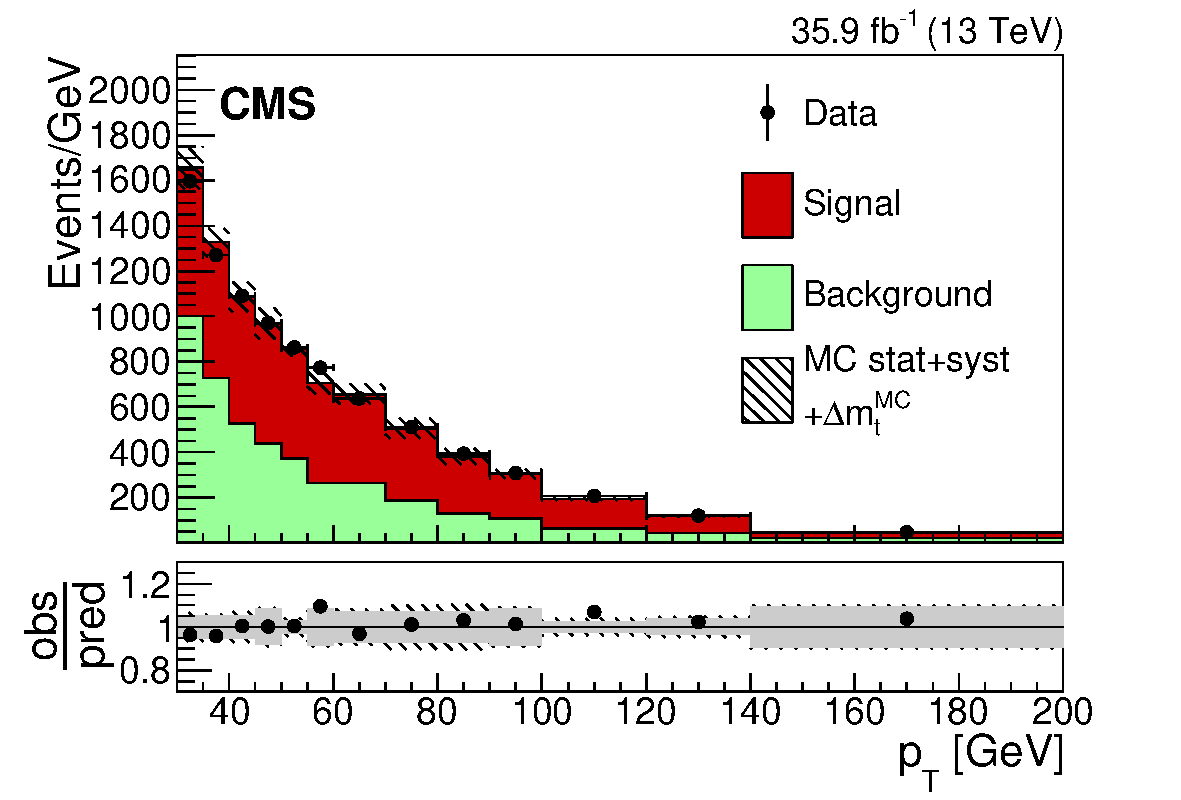
\includegraphics{Results/Figures/FitPlots/emu/lead_jet_pt_0,1_b_jets_step_8_postfit.pdf}}
    \resizebox{0.32 \textwidth}{!}{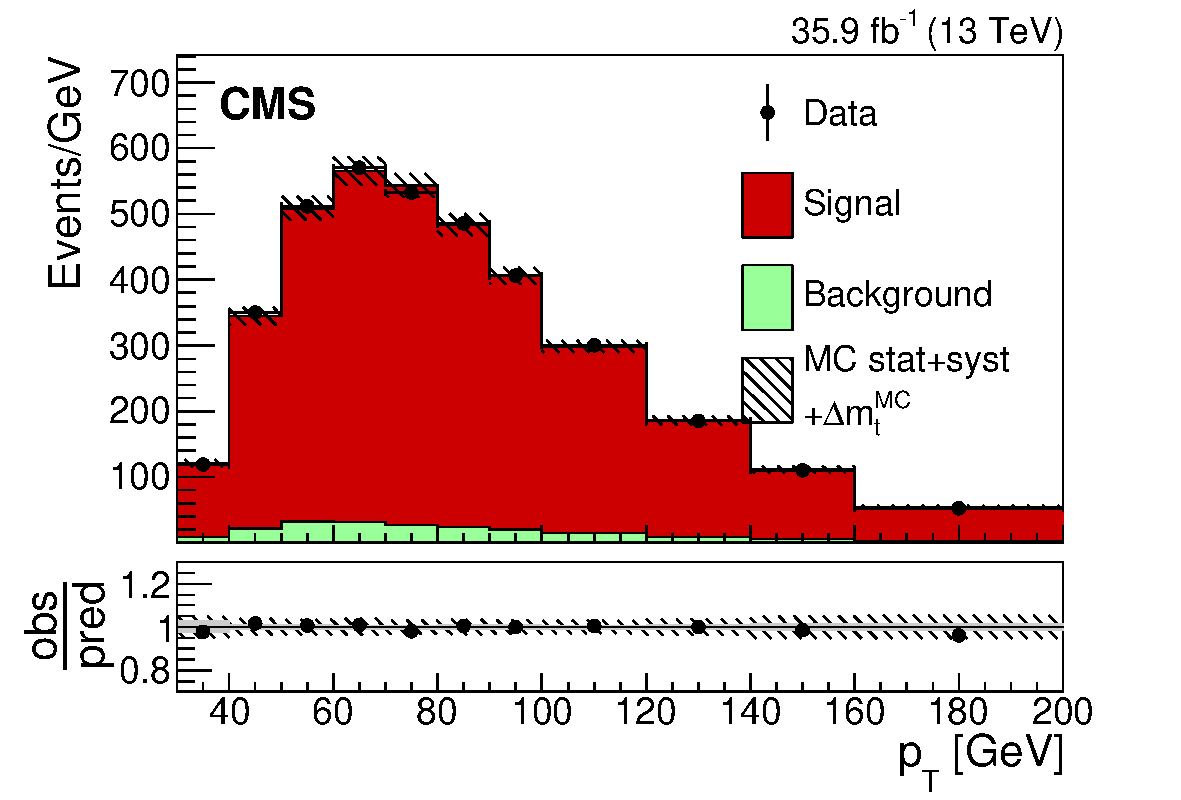
\includegraphics{Results/Figures/FitPlots/emu/lead_jet_pt_1,1_b_jets_step_8_postfit.pdf}}
    \resizebox{0.32 \textwidth}{!}{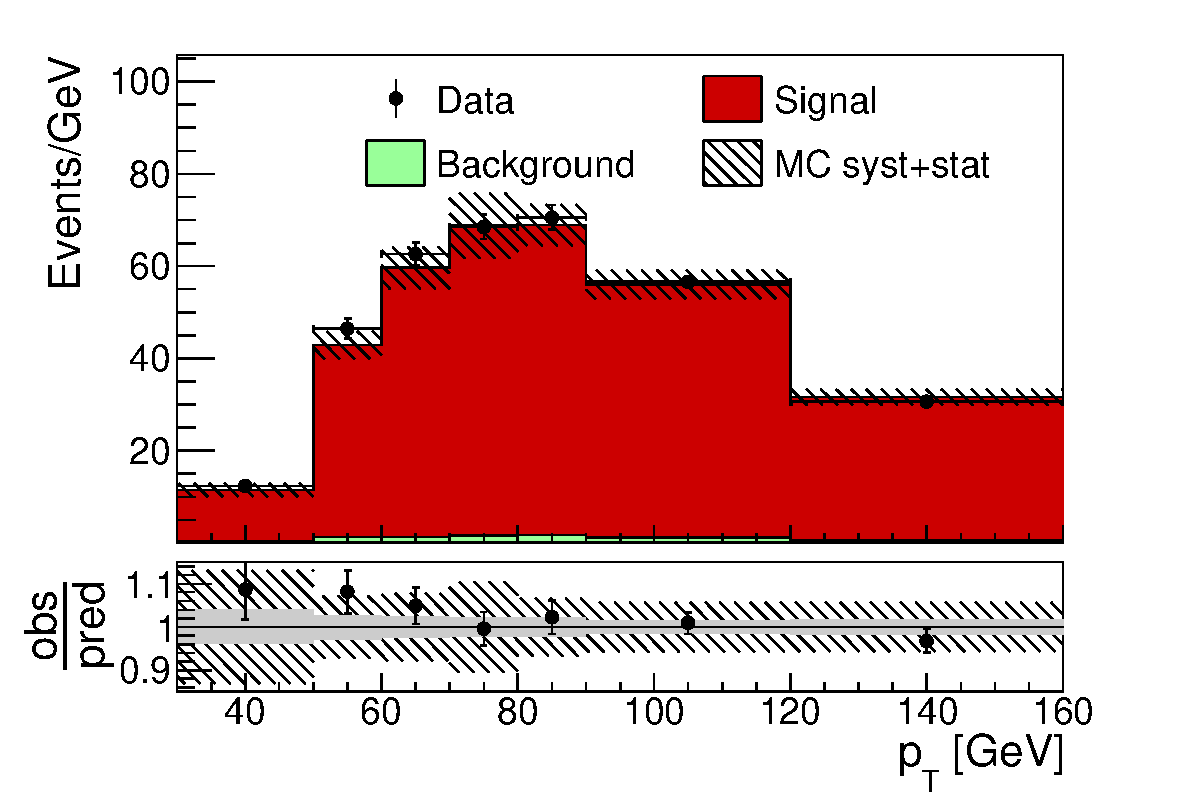
\includegraphics{Results/Figures/FitPlots/emu/lead_jet_pt_2,1_b_jets_step_8_postfit.pdf}}

    \resizebox{0.32 \textwidth}{!}{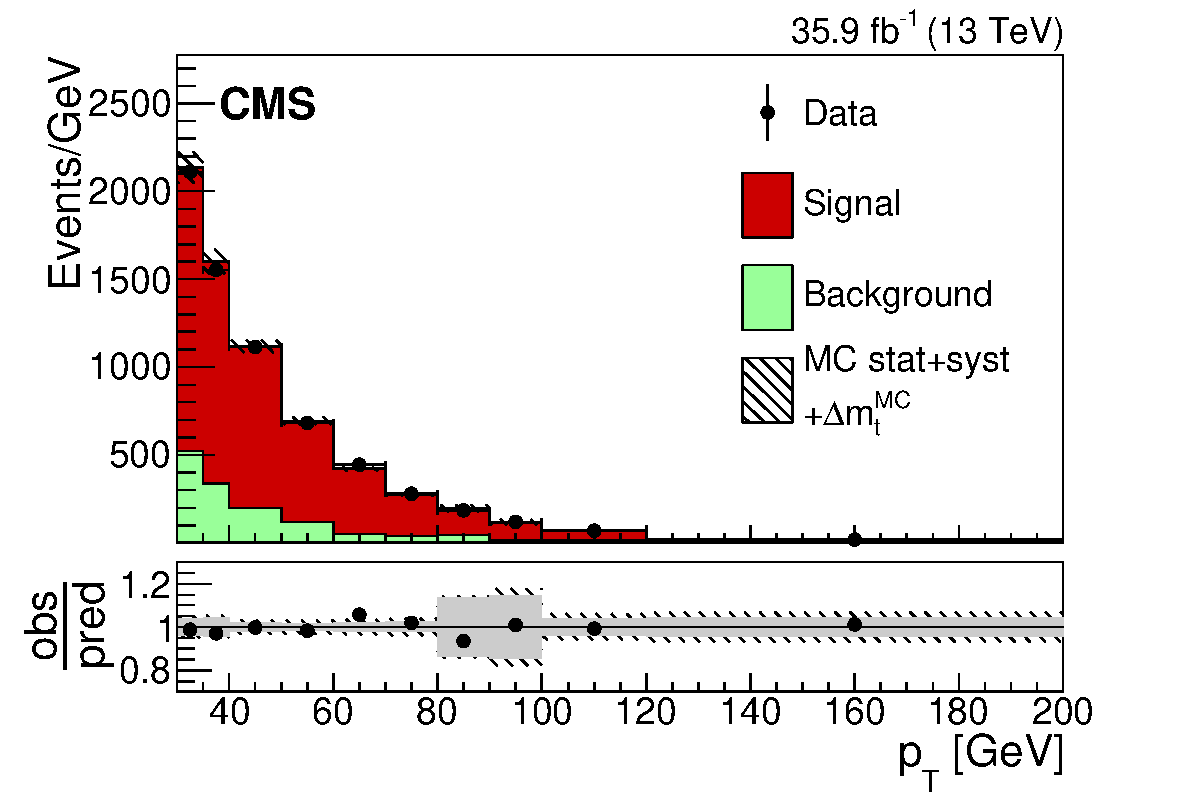
\includegraphics{Results/Figures/FitPlots/emu/second_jet_pt_0,2_b_jets_step_8_postfit.pdf}}
    \resizebox{0.32 \textwidth}{!}{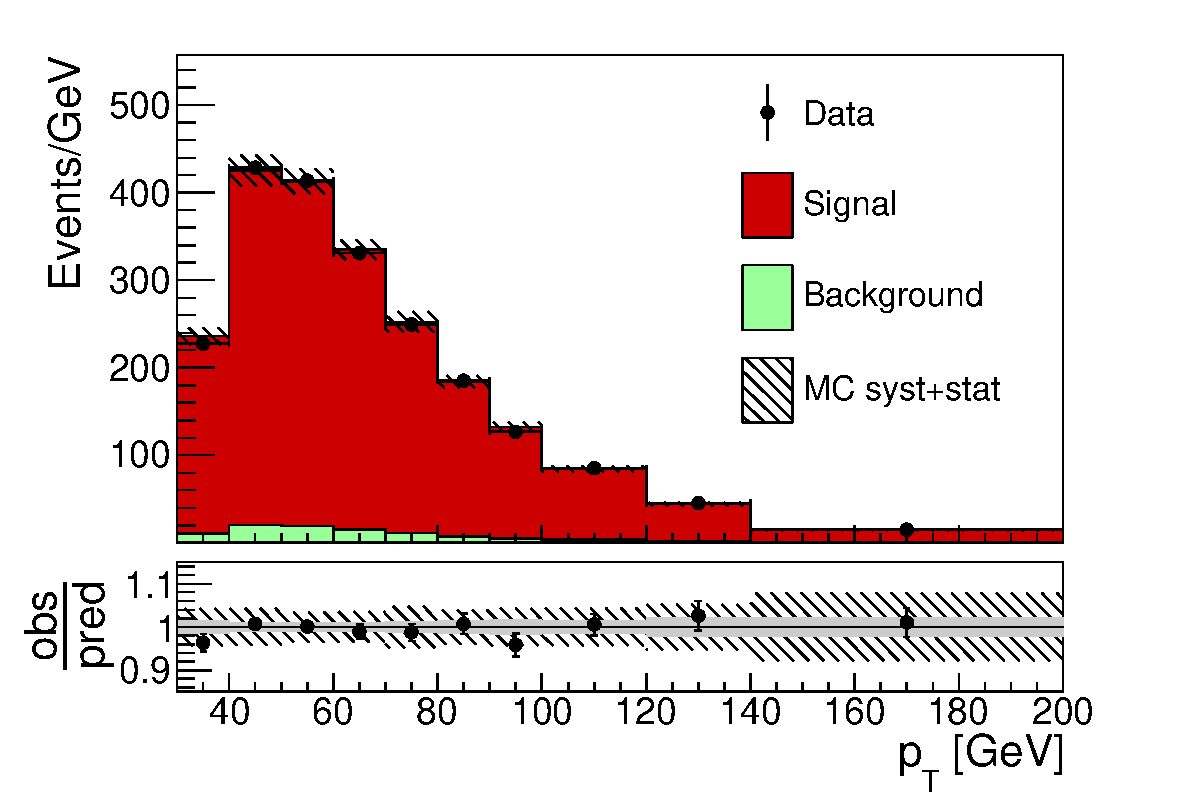
\includegraphics{Results/Figures/FitPlots/emu/second_jet_pt_1,2_b_jets_step_8_postfit.pdf}}
    \resizebox{0.32 \textwidth}{!}{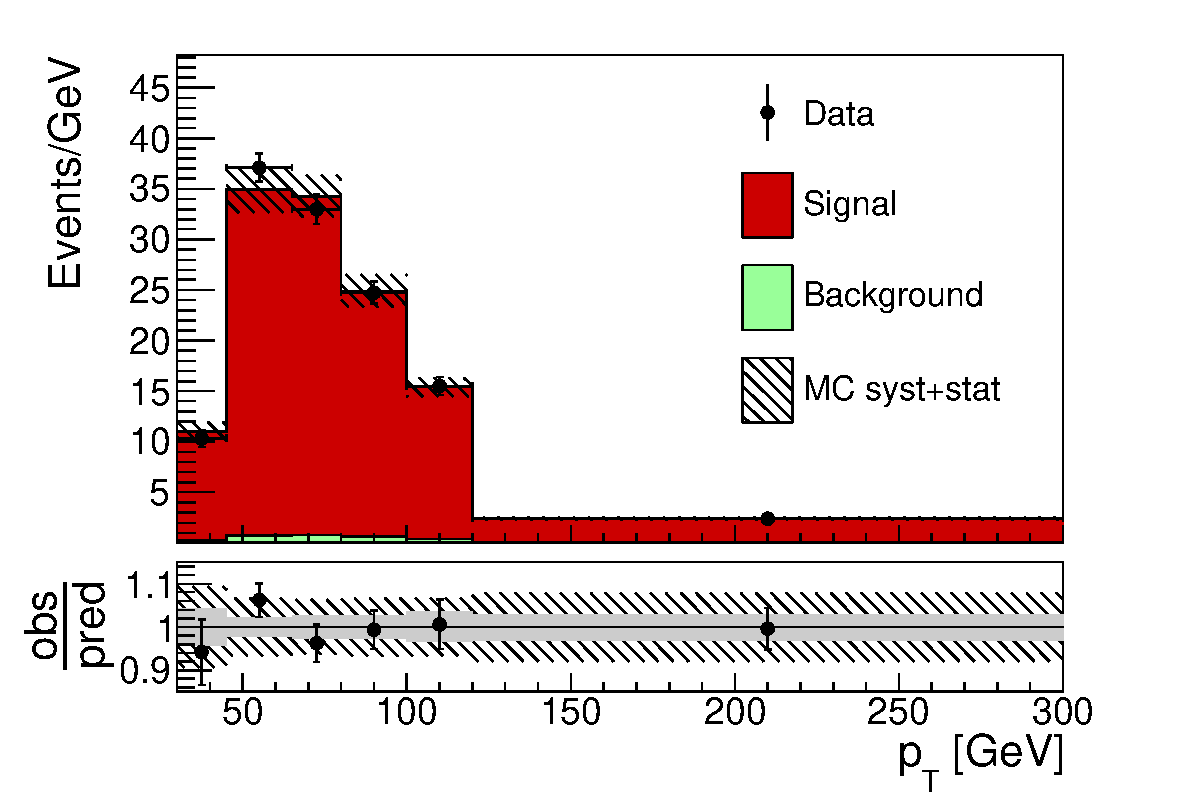
\includegraphics{Results/Figures/FitPlots/emu/second_jet_pt_2,2_b_jets_step_8_postfit.pdf}}    

    \resizebox{0.32 \textwidth}{!}{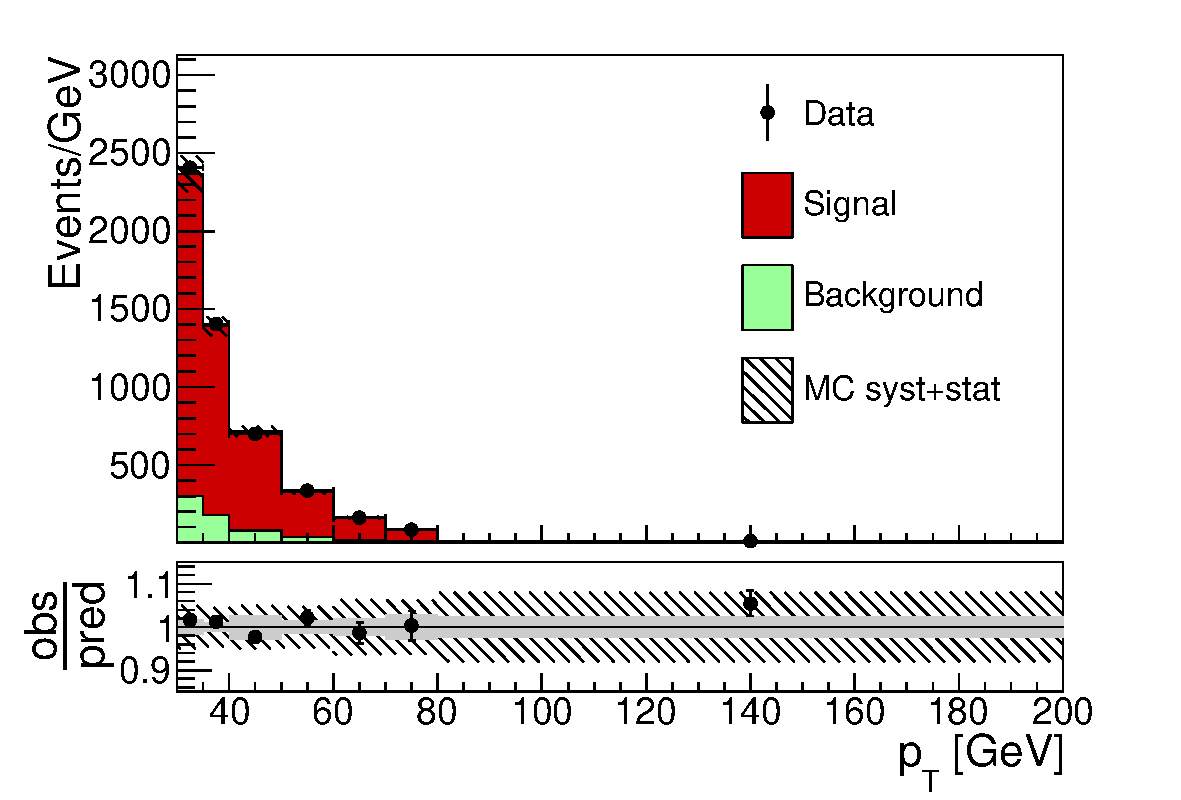
\includegraphics{Results/Figures/FitPlots/emu/third_jet_pt_0,3_b_jets_step_8_postfit.pdf}}
    \resizebox{0.32 \textwidth}{!}{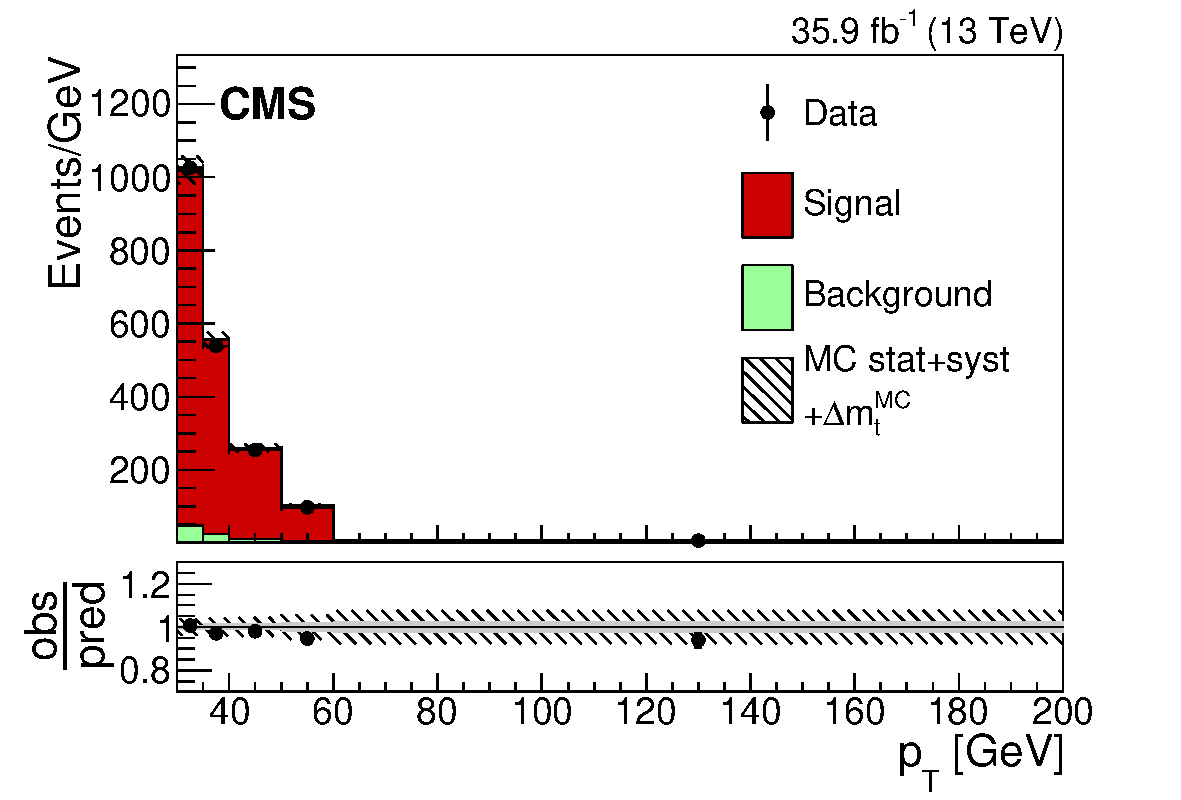
\includegraphics{Results/Figures/FitPlots/emu/third_jet_pt_1,3_b_jets_step_8_postfit.pdf}}
    \resizebox{0.32 \textwidth}{!}{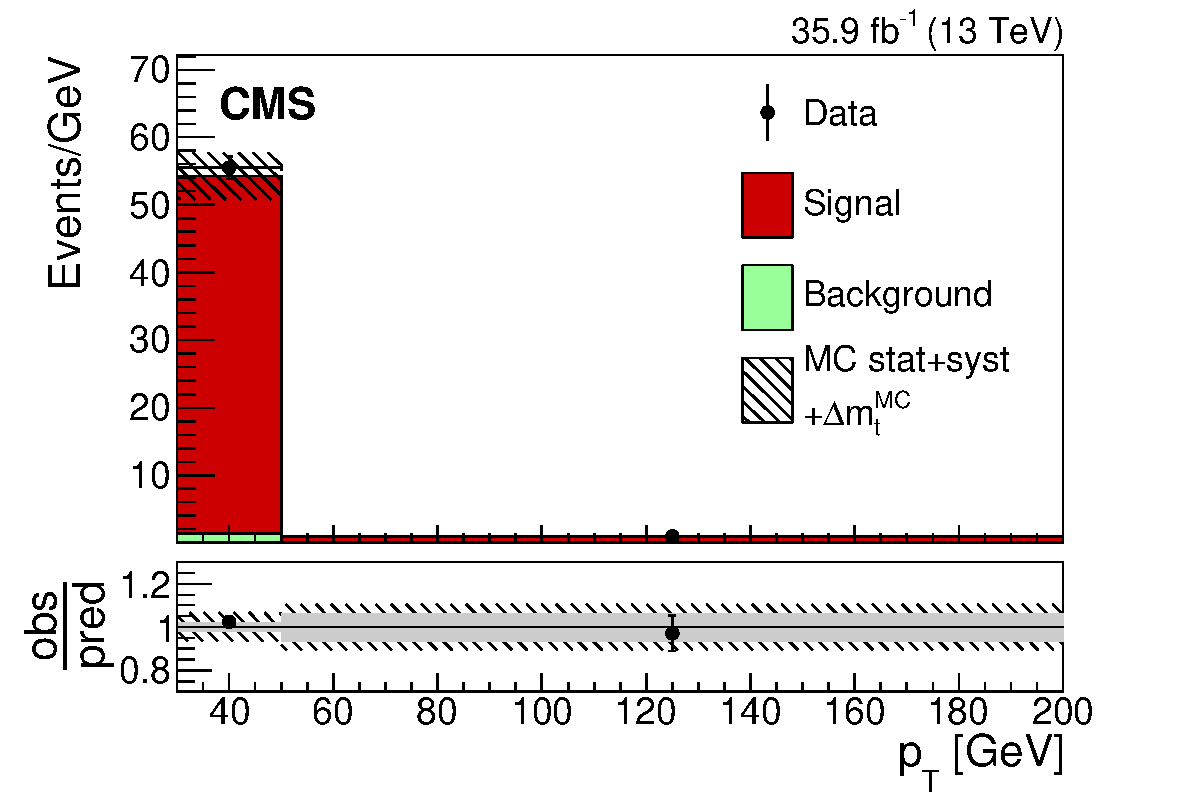
\includegraphics{Results/Figures/FitPlots/emu/third_jet_pt_2,3_b_jets_step_8_postfit.pdf}}   

\caption{Fitted Distributions (\emu channel) for events with zero as well as three or
  more b-tagged jets (left column): Total event yield for zero (top) and the trailing jet pt for one (second from top),
  two (second from bottom) or three or more (bottom) additional jets. The same for events with one
  b-tagged jet (middle column) and two b-tagged jets (right column) are
  shown below.   
  The hatched bands correspond to the total uncertainty on the sum of
  the predicted yields. The ratios of data to the sum of the
  predicted yields are shown at the bottom of each plot. Here, the solid
  gray band represents the contribution of the statistical uncertainty.   
       \label{fig:lh_emu_postfitdistr8}}
  \end{center}
\end{figure}

\begin{figure}[htbp!]
  \begin{center}

    \resizebox{0.32 \textwidth}{!}{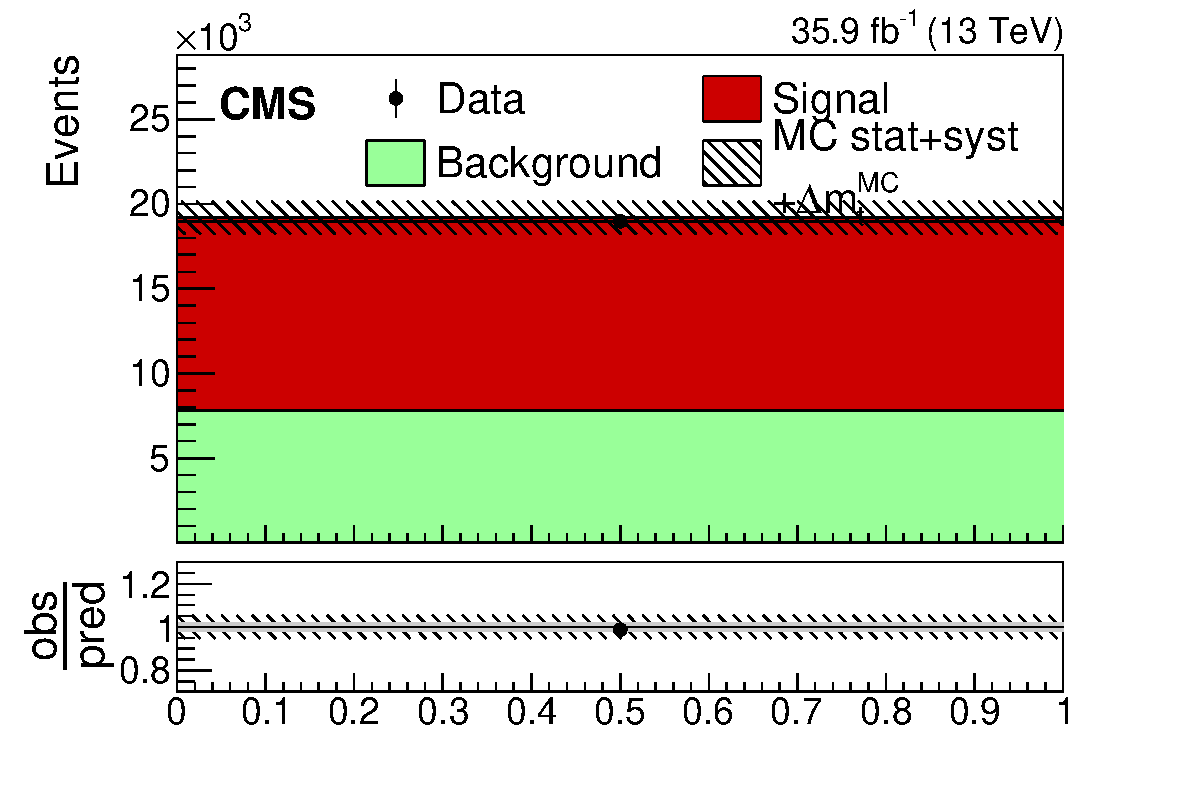
\includegraphics{Results/Figures/FitPlots/mumu/total_1,0_b_jets_step_8_postfit.pdf}}
    \resizebox{0.32 \textwidth}{!}{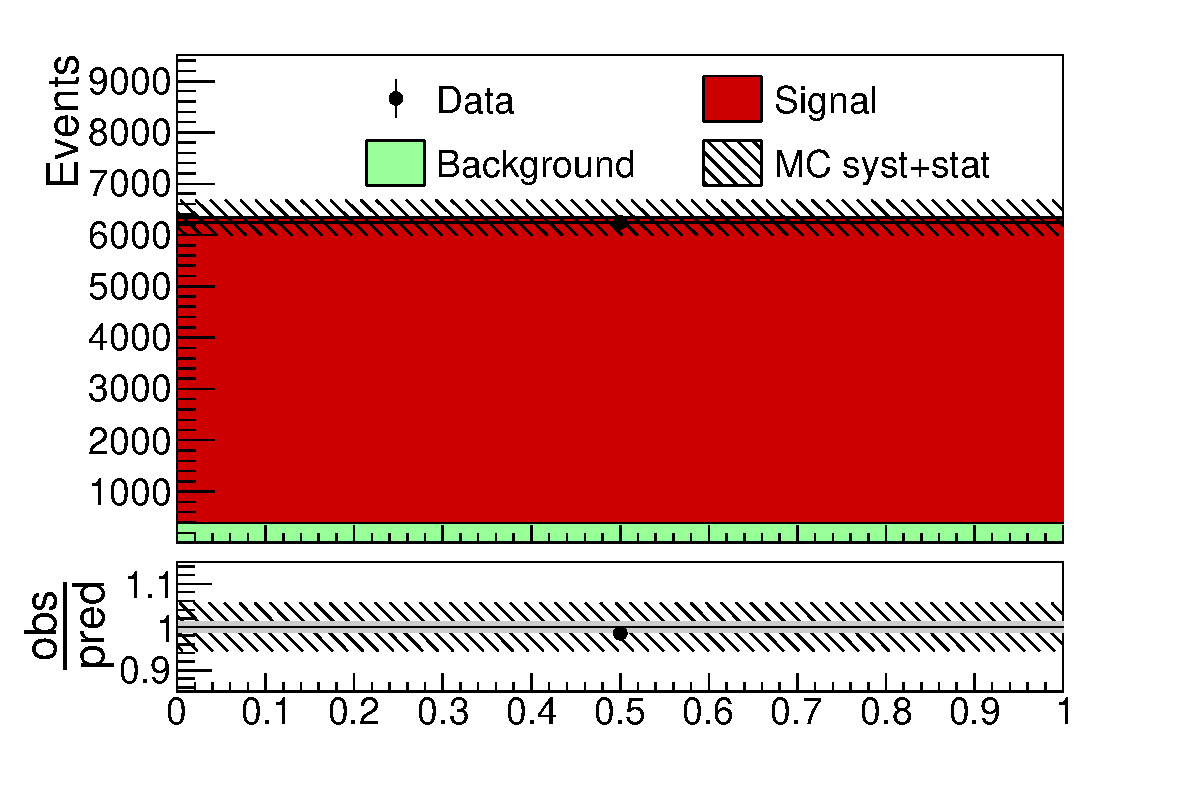
\includegraphics{Results/Figures/FitPlots/mumu/total_2,0_b_jets_step_8_postfit.pdf}}\\


    \resizebox{0.32 \textwidth}{!}{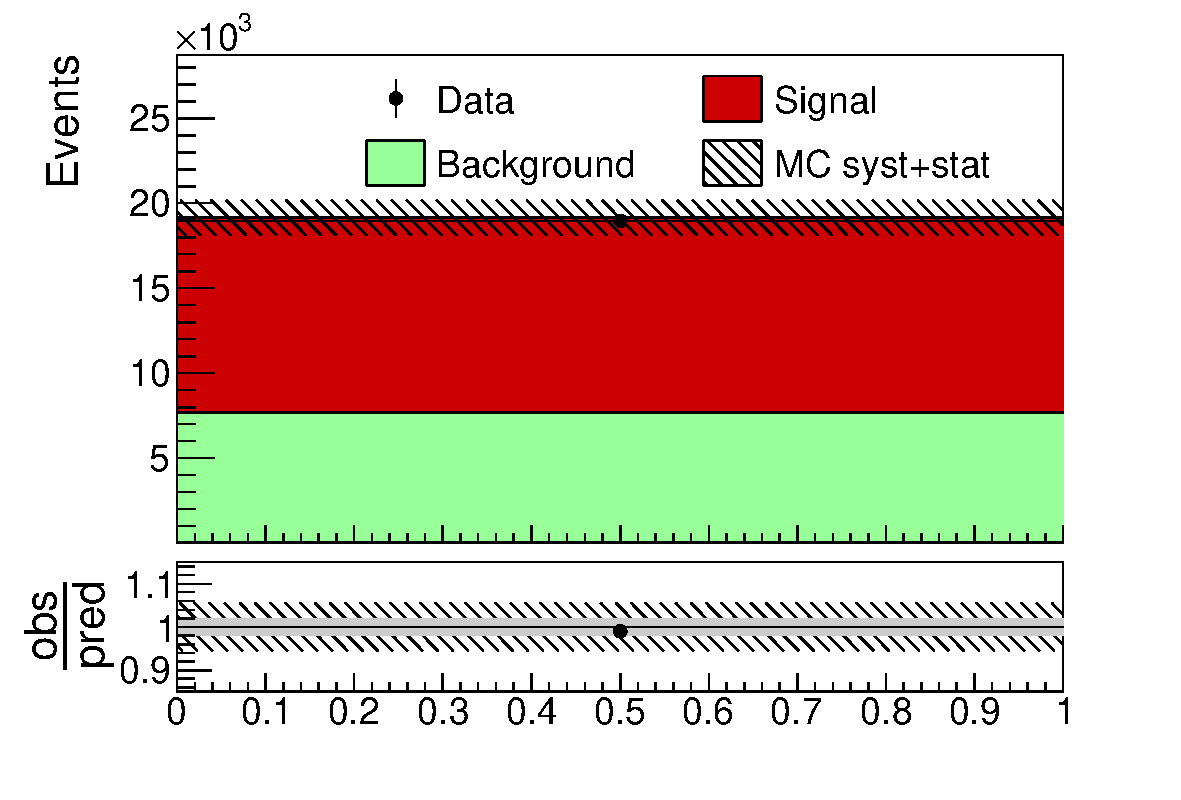
\includegraphics{Results/Figures/FitPlots/mumu/total_1,1_b_jets_step_8_postfit.pdf}}
    \resizebox{0.32 \textwidth}{!}{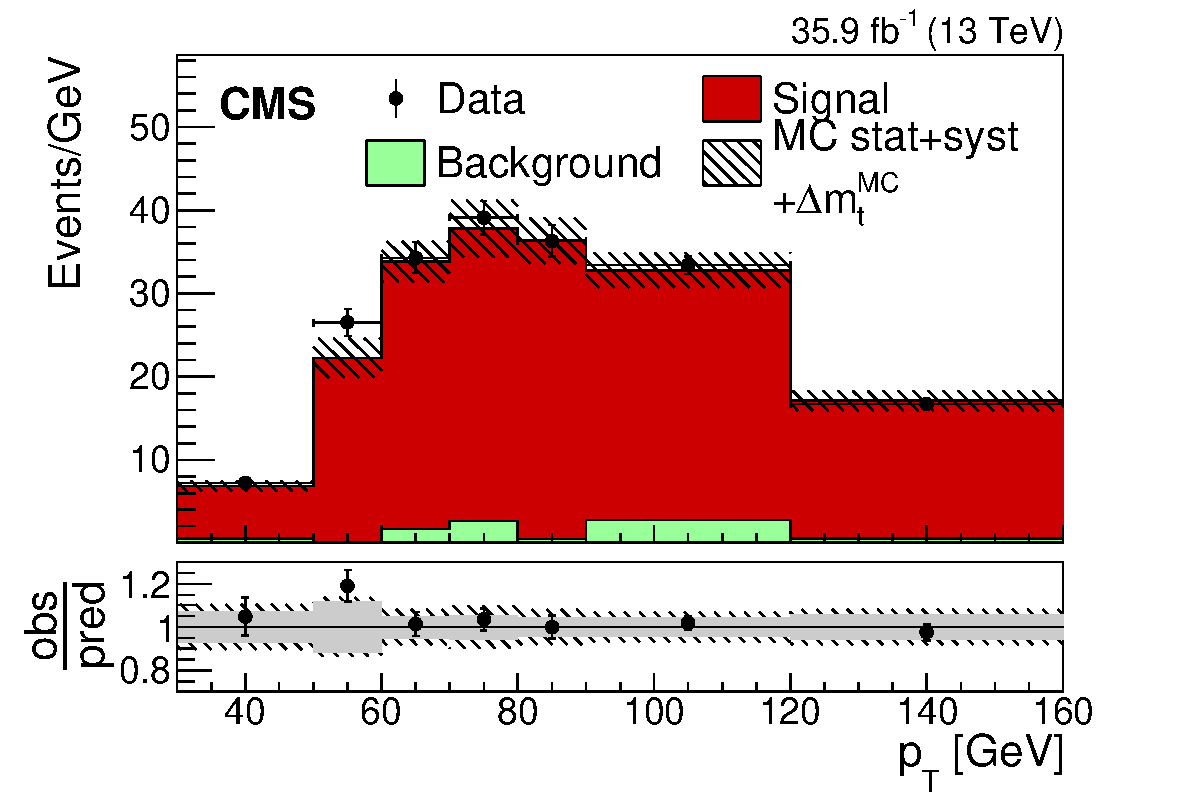
\includegraphics{Results/Figures/FitPlots/mumu/lead_jet_pt_2,1_b_jets_step_8_postfit.pdf}}\\


    \resizebox{0.32 \textwidth}{!}{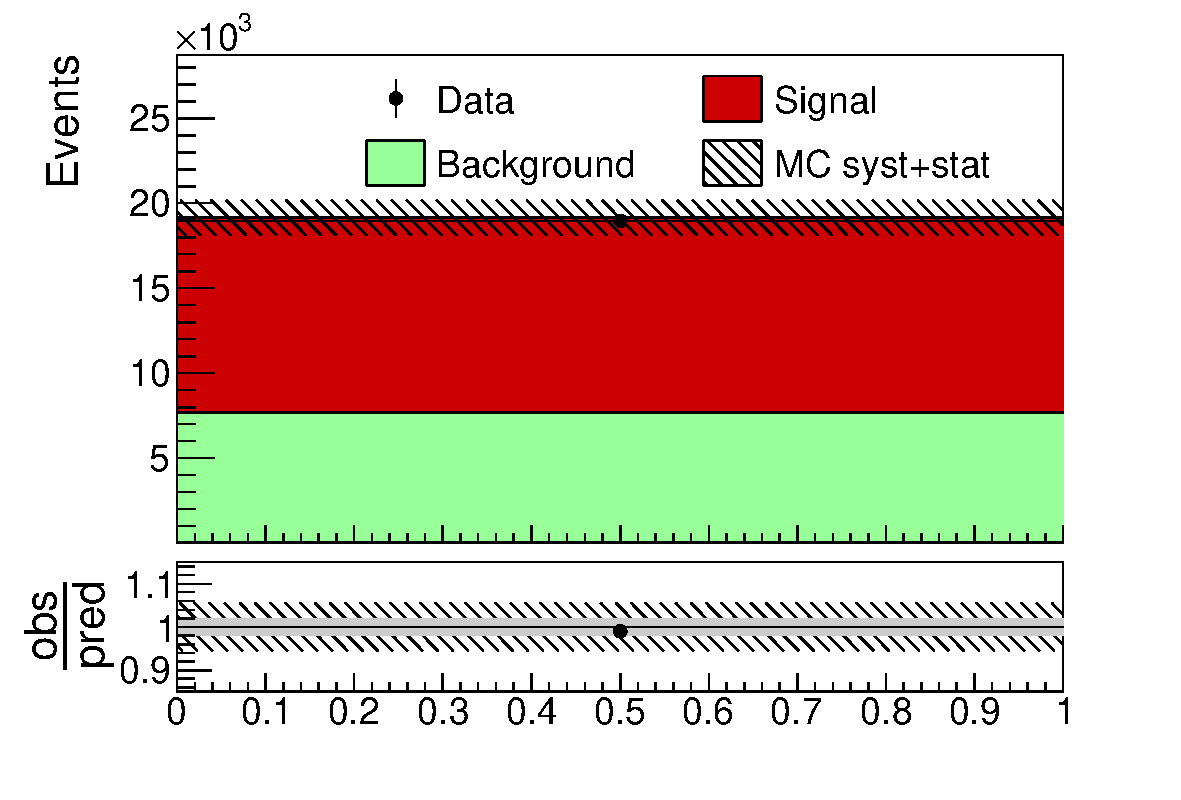
\includegraphics{Results/Figures/FitPlots/mumu/total_1,2_b_jets_step_8_postfit.pdf}}
    \resizebox{0.32 \textwidth}{!}{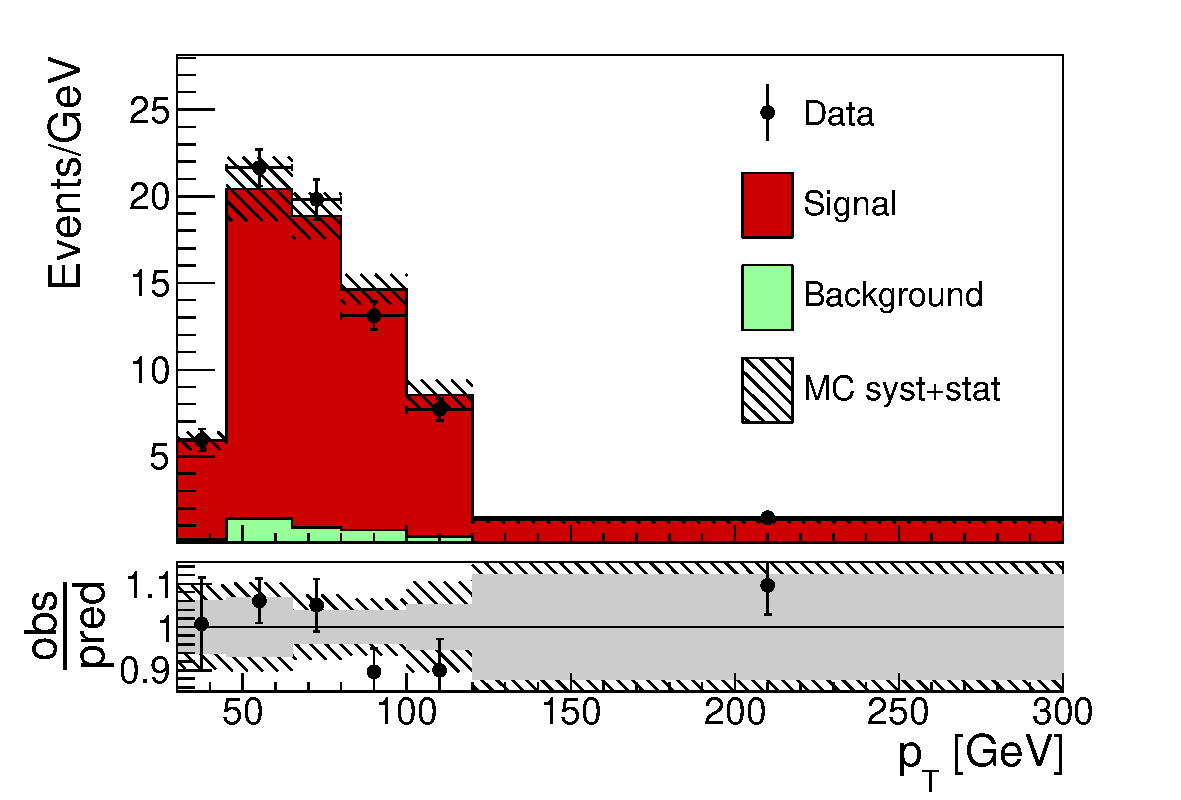
\includegraphics{Results/Figures/FitPlots/mumu/second_jet_pt_2,2_b_jets_step_8_postfit.pdf}}  \\  


    \resizebox{0.32 \textwidth}{!}{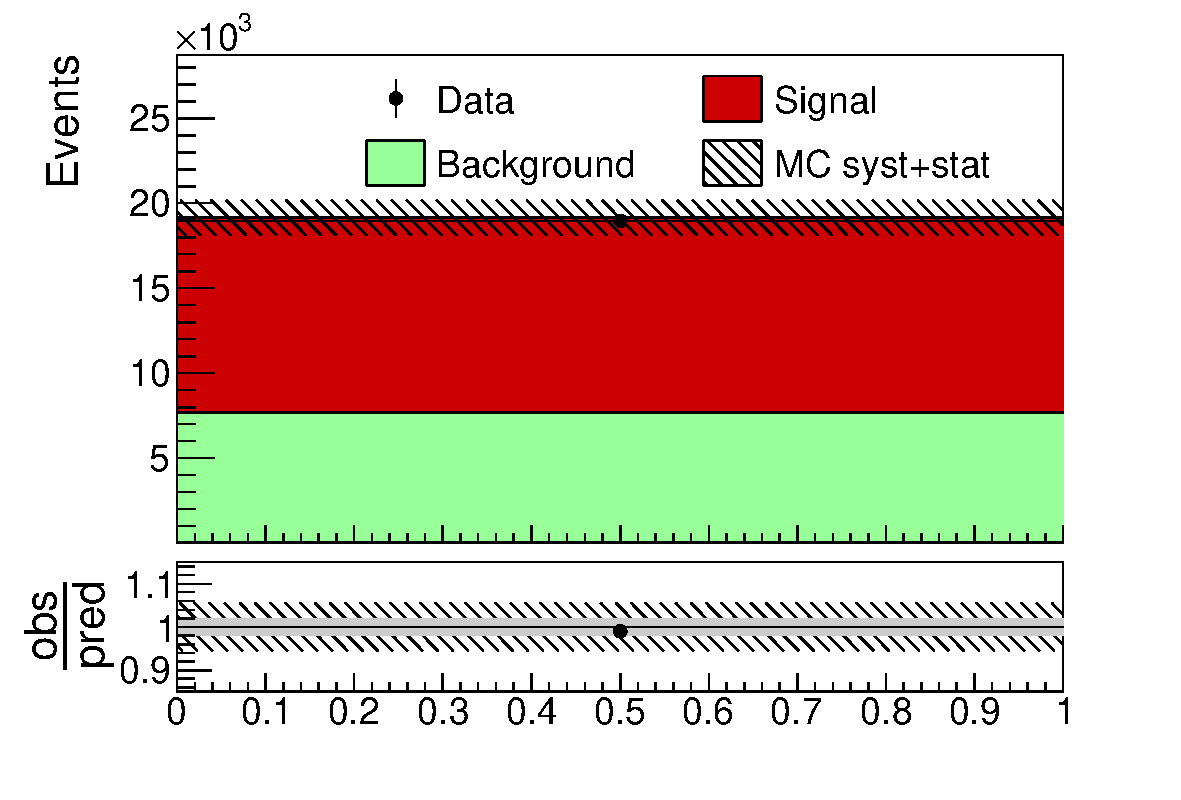
\includegraphics{Results/Figures/FitPlots/mumu/total_1,3_b_jets_step_8_postfit.pdf}}
    \resizebox{0.32 \textwidth}{!}{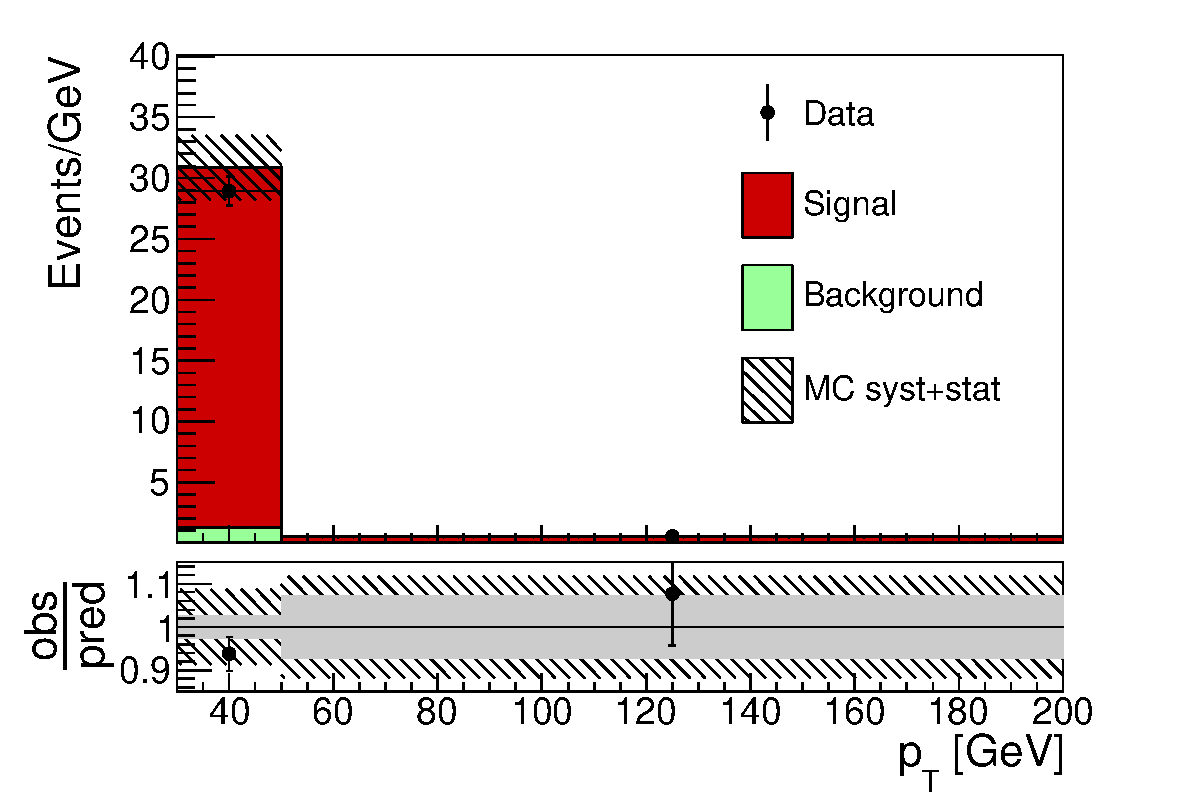
\includegraphics{Results/Figures/FitPlots/mumu/third_jet_pt_2,3_b_jets_step_8_postfit.pdf}}   

\caption{Fitted distributions (\mumu channel): 
  The left column shows events with one b-tagged jet and the total event yield for events with zero (top), one (second from top)
  two (second from bottom) or three or more additional jets (bottom).
  The right column shows events with two b-tagged jets and the total yield for events with zero additional jets (top),
  the trailing jet pt for one (second from top),
  two (second from bottom) or three or more (bottom) additional jets.
  The hatched bands correspond to the total uncertainty on the sum of
  the predicted yields. The ratios of data to the sum of the
  predicted yields are shown at the bottom of each plot. Here, the solid
  gray band represents the contribution of the statistical uncertainty.  
       \label{fig:lh_mumu_postfitdistr8}}
  \end{center}
\end{figure}

\begin{figure}[htbp!]
  \begin{center}
    \resizebox{0.32 \textwidth}{!}{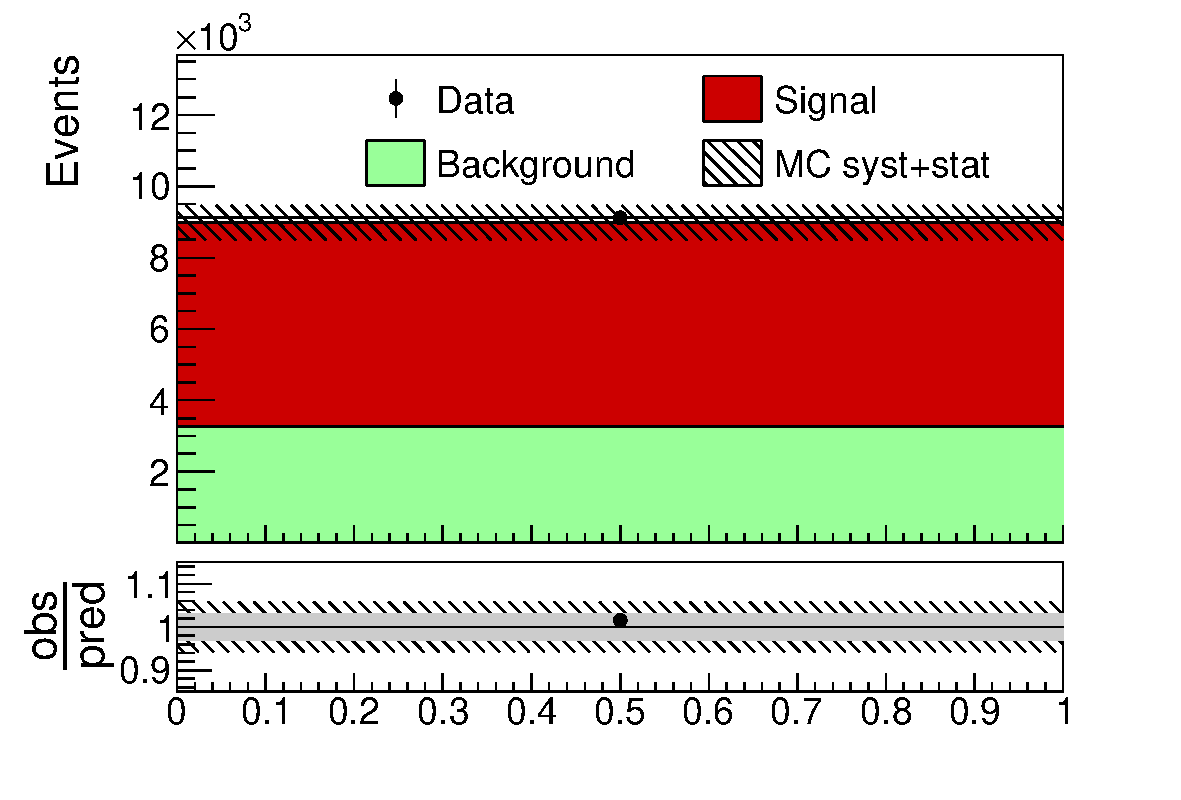
\includegraphics{Results/Figures/FitPlots/ee/total_1,0_b_jets_step_8_postfit.pdf}}
    \resizebox{0.32 \textwidth}{!}{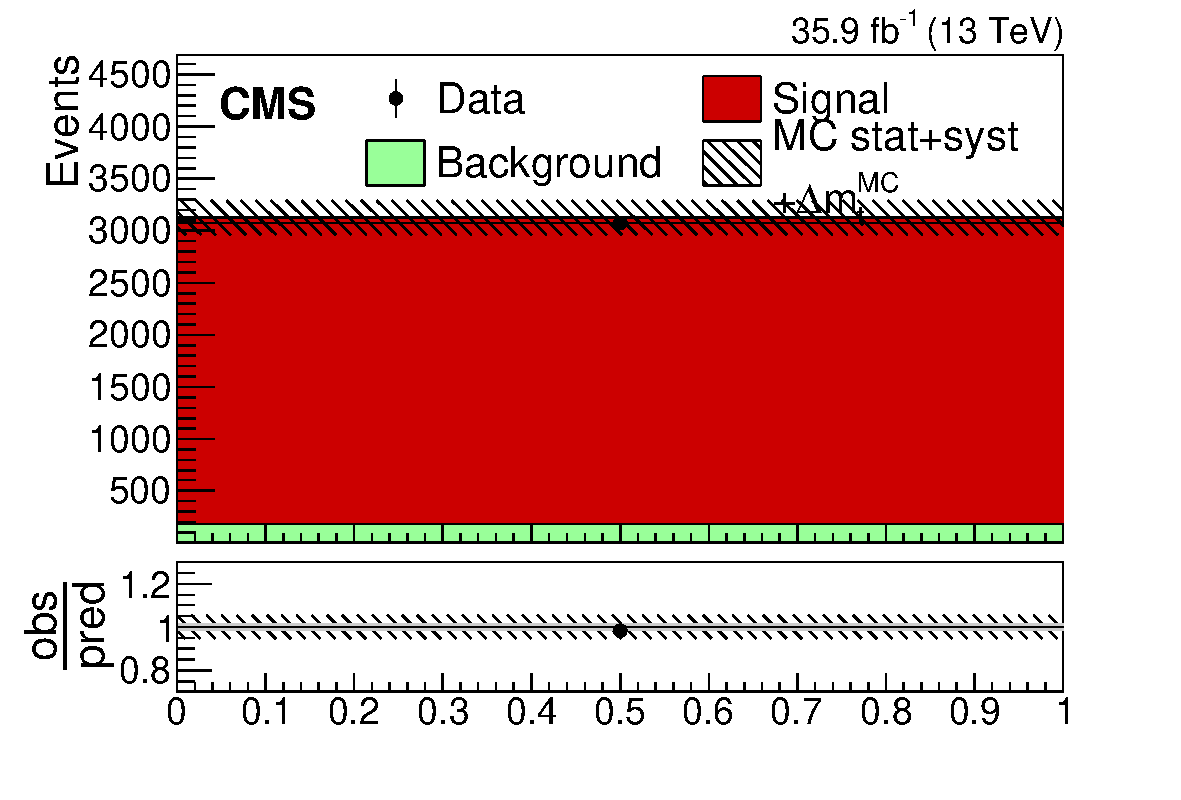
\includegraphics{Results/Figures/FitPlots/ee/total_2,0_b_jets_step_8_postfit.pdf}}\\

    \resizebox{0.32 \textwidth}{!}{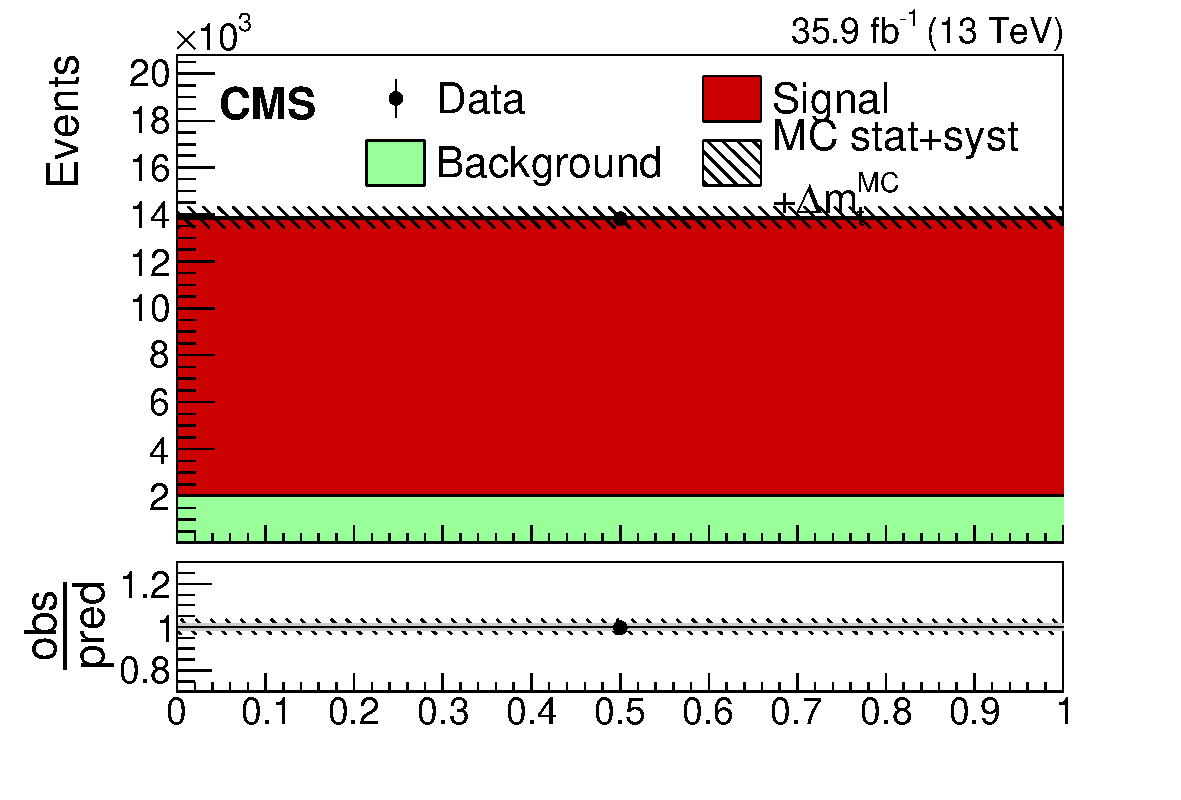
\includegraphics{Results/Figures/FitPlots/ee/total_1,1_b_jets_step_8_postfit.pdf}}
    \resizebox{0.32 \textwidth}{!}{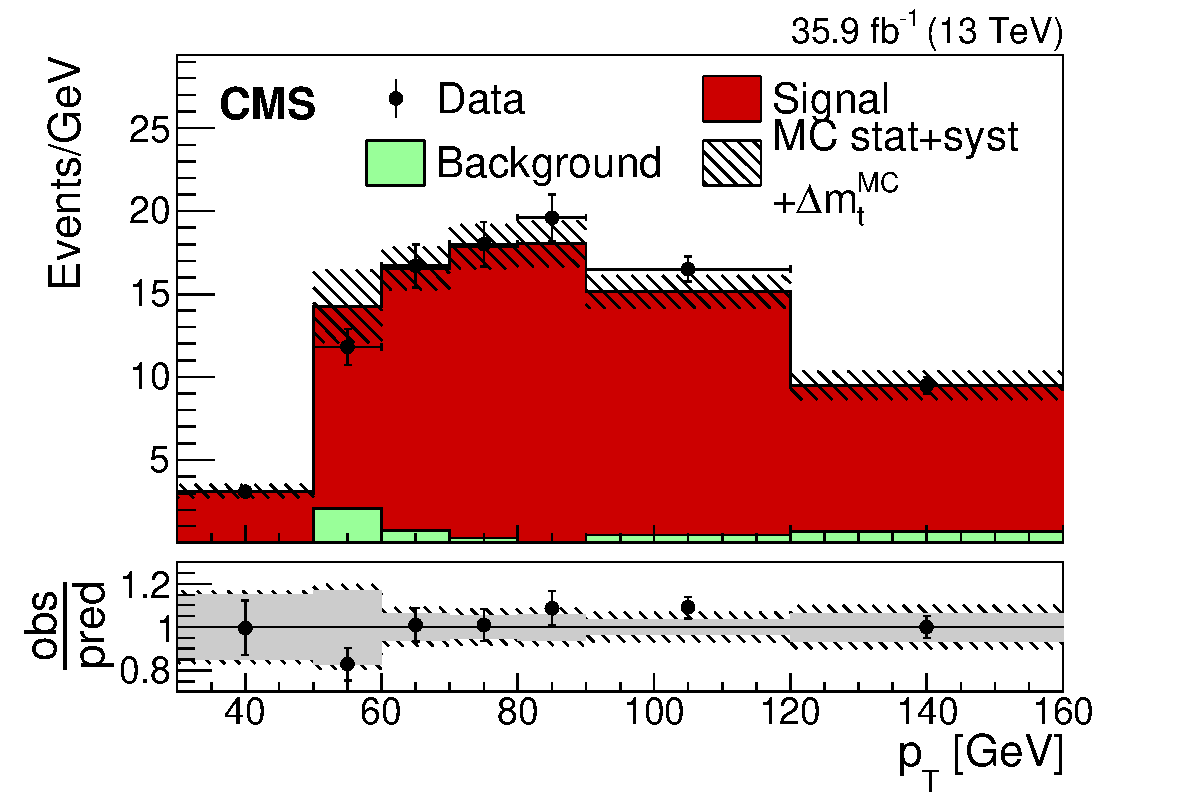
\includegraphics{Results/Figures/FitPlots/ee/lead_jet_pt_2,1_b_jets_step_8_postfit.pdf}}\\

    \resizebox{0.32 \textwidth}{!}{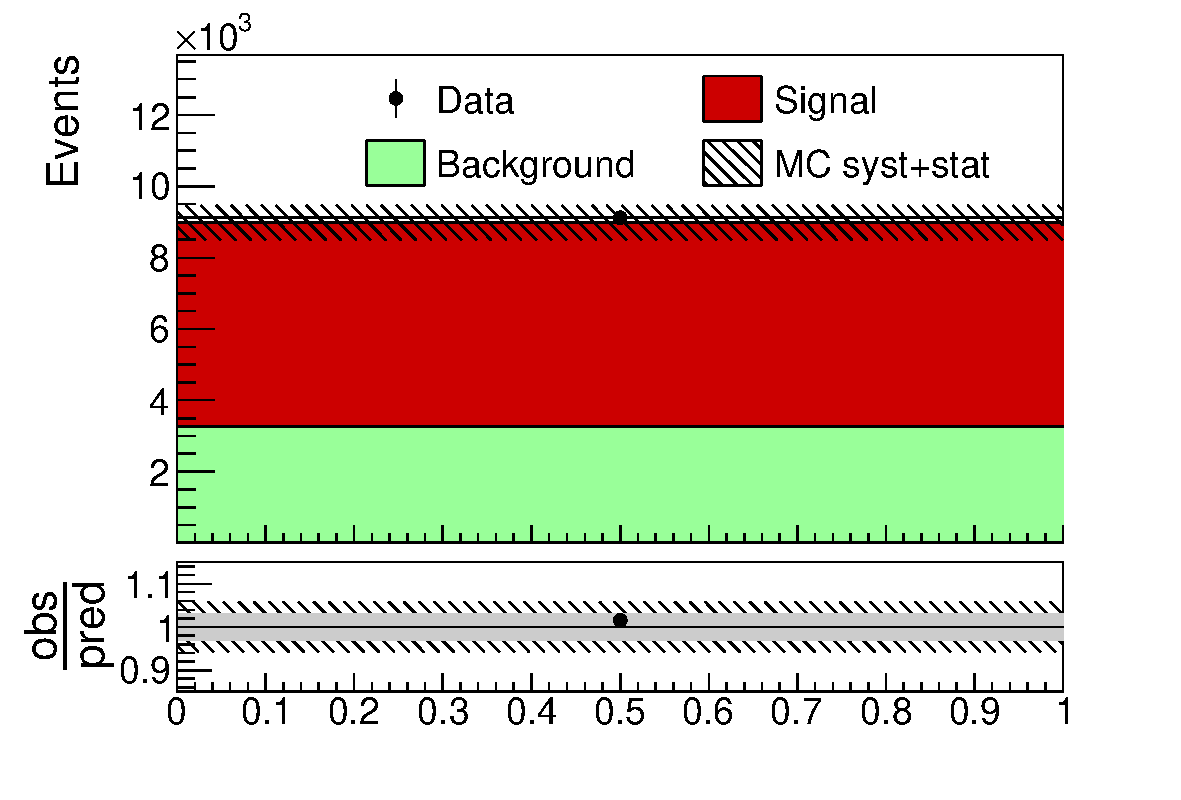
\includegraphics{Results/Figures/FitPlots/ee/total_1,2_b_jets_step_8_postfit.pdf}}
    \resizebox{0.32 \textwidth}{!}{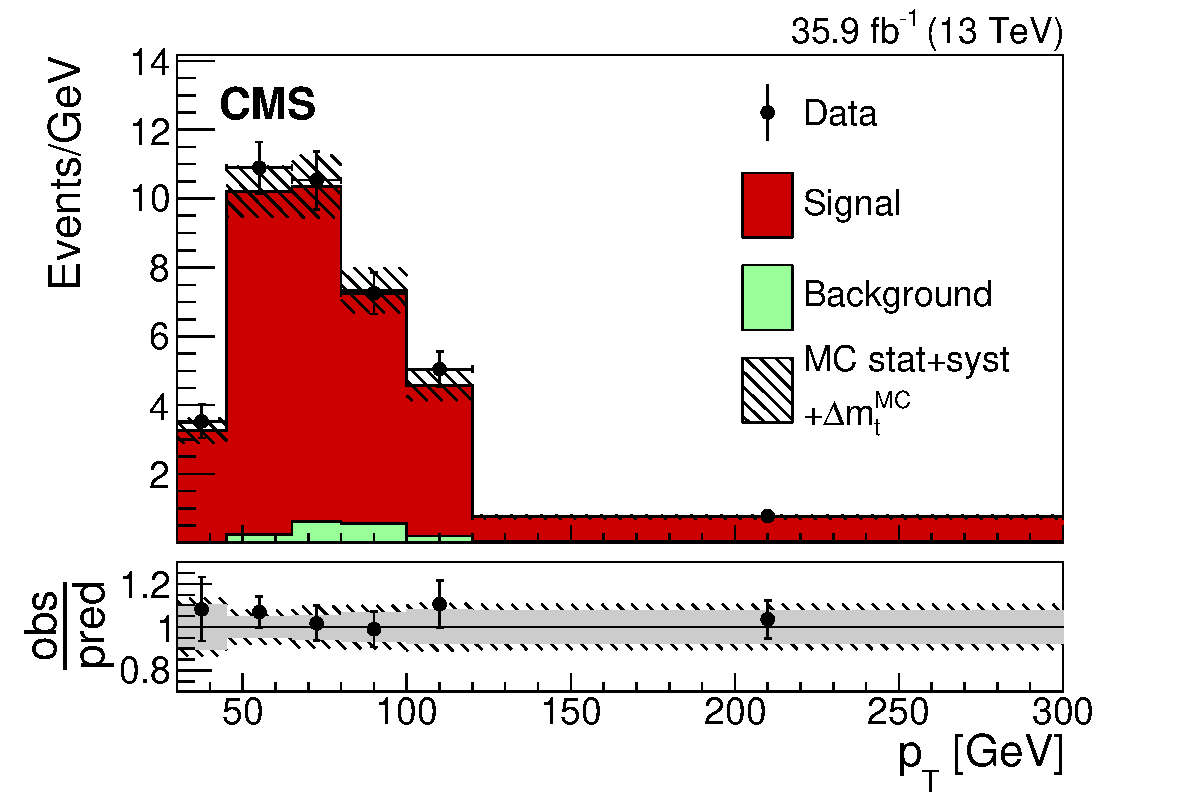
\includegraphics{Results/Figures/FitPlots/ee/second_jet_pt_2,2_b_jets_step_8_postfit.pdf}} \\   

    \resizebox{0.32 \textwidth}{!}{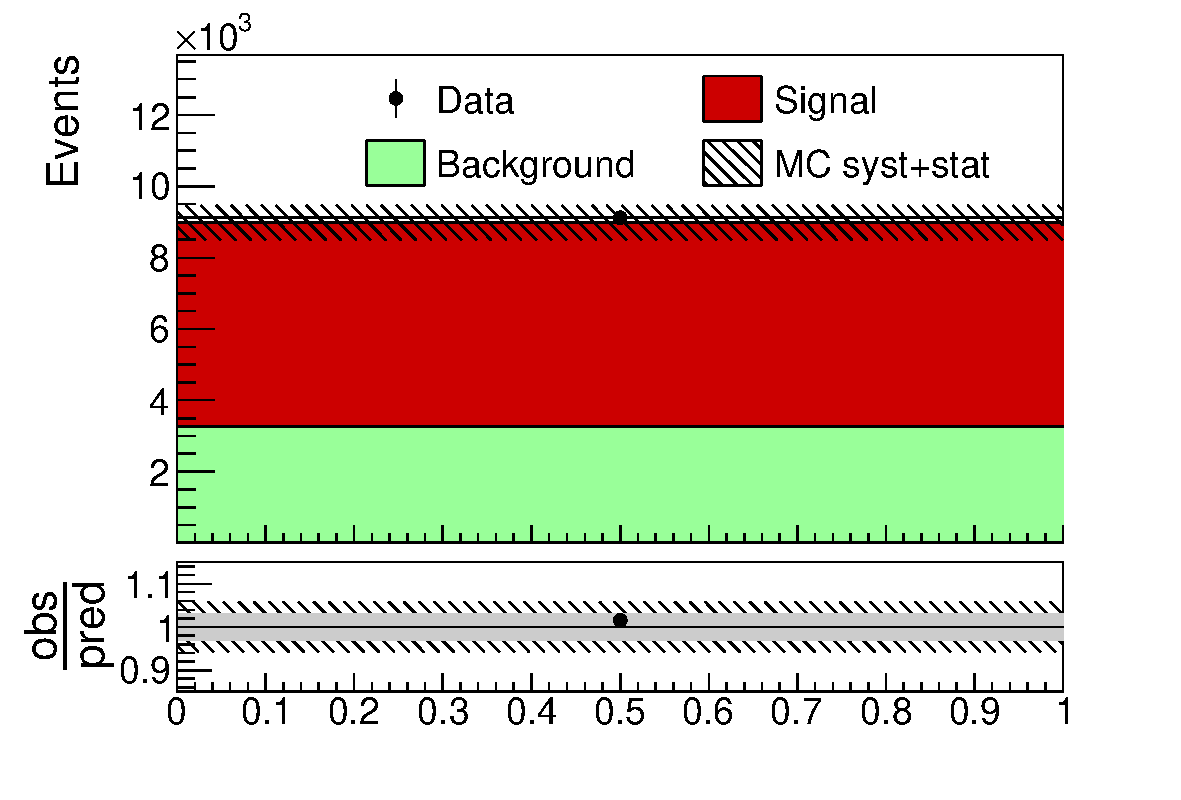
\includegraphics{Results/Figures/FitPlots/ee/total_1,3_b_jets_step_8_postfit.pdf}}
    \resizebox{0.32 \textwidth}{!}{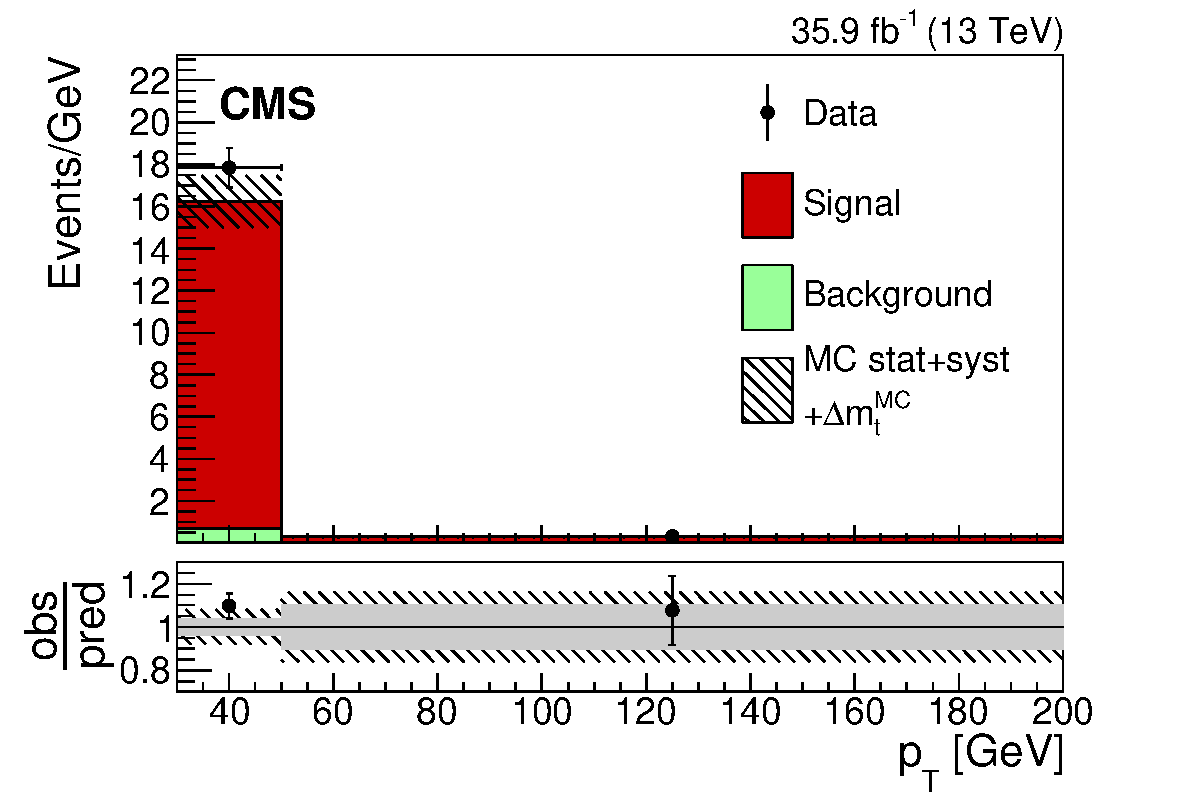
\includegraphics{Results/Figures/FitPlots/ee/third_jet_pt_2,3_b_jets_step_8_postfit.pdf}}   

\caption{Fitted distributions (\ee channel): 
  The left column shows events with one b-tagged jet and the total event yield for events with zero (top), one (second from top)
  two (second from bottom) or three or more additional jets (bottom).
  The right column shows events with two b-tagged jets and the total yield for events with zero additional jets (top),
  the trailing jet pt for one (second from top),
  two (second from bottom) or three or more (bottom) additional jets.
  The hatched bands correspond to the total uncertainty on the sum of
  the predicted yields. The ratios of data to the sum of the
  predicted yields are shown at the bottom of each plot. Here, the solid
  gray band represents the contribution of the statistical uncertainty.  
       \label{fig:lh_ee_postfitdistr8}}
  \end{center}
\end{figure}

The plots show that simulation agrees with the data after applying the fitted parameters.
The agreement can be expected after a succesfull git, but its still
The plotted uncertainties are smaller compared to the plots showing the non-constrained uncertainties in Figure \ref{fig:xsec_emu_inputdistr},\ref{fig:xsec_mumu_inputdistr} and \ref{fig:xsec_ee_inputdistr}.


\section{Breakdown of systematic uncertainties}
\label{sec:results_uncert}


\section{Comparison to theory predictions and previous results}
\label{results_comp}